\documentclass[a4paper, 12pt]{article}

\usepackage{authblk} % Title, Author and affiliation formatting
\usepackage[utf8]{inputenc} % Encoding
\usepackage{datetime} % Time and Date formatting
\usepackage[portuguese]{babel}

\usepackage{csquotes}

\usepackage{biblatex} % Bibliography management
\addbibresource{refs.bib}

\usepackage{hyperref} % links
\hypersetup{
colorlinks = true,
linkcolor = blue,
urlcolor = blue,
pdftitle = {Iniciando com Latex},
pdfauthor = {Kauê Fraga Rodrigues},
pdfpagemode = FullScreen,
}

\usepackage{roboto}
\usepackage[T1]{fontenc}

\usepackage{graphicx} % Images
\usepackage{setspace}

% Customização -----

% geometry - sets paper size and margins
\usepackage{geometry}
\geometry{
top = 3cm,
bottom = 2cm,
left = 3cm,
right = 2cm,
}

% line height
\renewcommand{\baselinestretch}{1.15}

% parskip and parindent
\setlength{\parindent}{0pt} % tamanho do espaço para iniciar o paragrafo
\setlength{\parskip}{0.8em} % espaço entre os paragrafos

% ------------------

\usepackage{amsmath, amssymb, amsthm}

\title{\vspace{-3.5cm}\huge{Iniciando com Latex}}
\author{\vspace{-3mm}Kauê Fraga Rodrigues}
\date{\vspace{-0.5cm}\today}

\renewcommand{\familydefault}{\sfdefault}

\setcounter{section}{0} %

\begin{document}
\maketitle

\section{Introdução} % You can prefix the braces with * and it won't have numbers
Olá! Meu nome é Kauê e eu gosto de escrever código.
Esse é um tutorial de \LaTeX para iniciantes. Nós vamos olhar como declarar
seções e subseções, equações e figures. Dê uma olhada em \cite{alves2003introduccao}

\section{Equações}
\subsection{Área de um Círculo}
Para calcular a área de um círculo, nós usamos esta equação:
\begin{equation}\label{AreaCirculo}
  A = \pi r^2
\end{equation}

\subsection{Área de um Cubo}
\begin{equation}\label{AreaCubo}
  A = 6 l^2
\end{equation}

A área do círculo é descrita pela equação~\ref{AreaCirculo}.
A área do cubo é dada pela equação~\ref{AreaCubo}.

\subsection{Luminosidade}
\begin{equation}\label{Luminosidade}
  L = 4 \pi r^2 \sigma T^4
\end{equation}

\newpage

\section{Matemática}
Começando outro tutorial, feito pelo Jake B.

\subsection{Escrevendo Equações}
Como eu escrevo uma equação com \LaTeX? \par
Em 1902, Einstein criou a seguinte equação: $E = mc^2$.

\begin{equation}
  \begin{split}
    A & = \frac{2}{4} \\
    A & = \frac{1}{2}
  \end{split}
\end{equation}

\subsection{Imagens}
\begin{figure}[h]
  \centering
  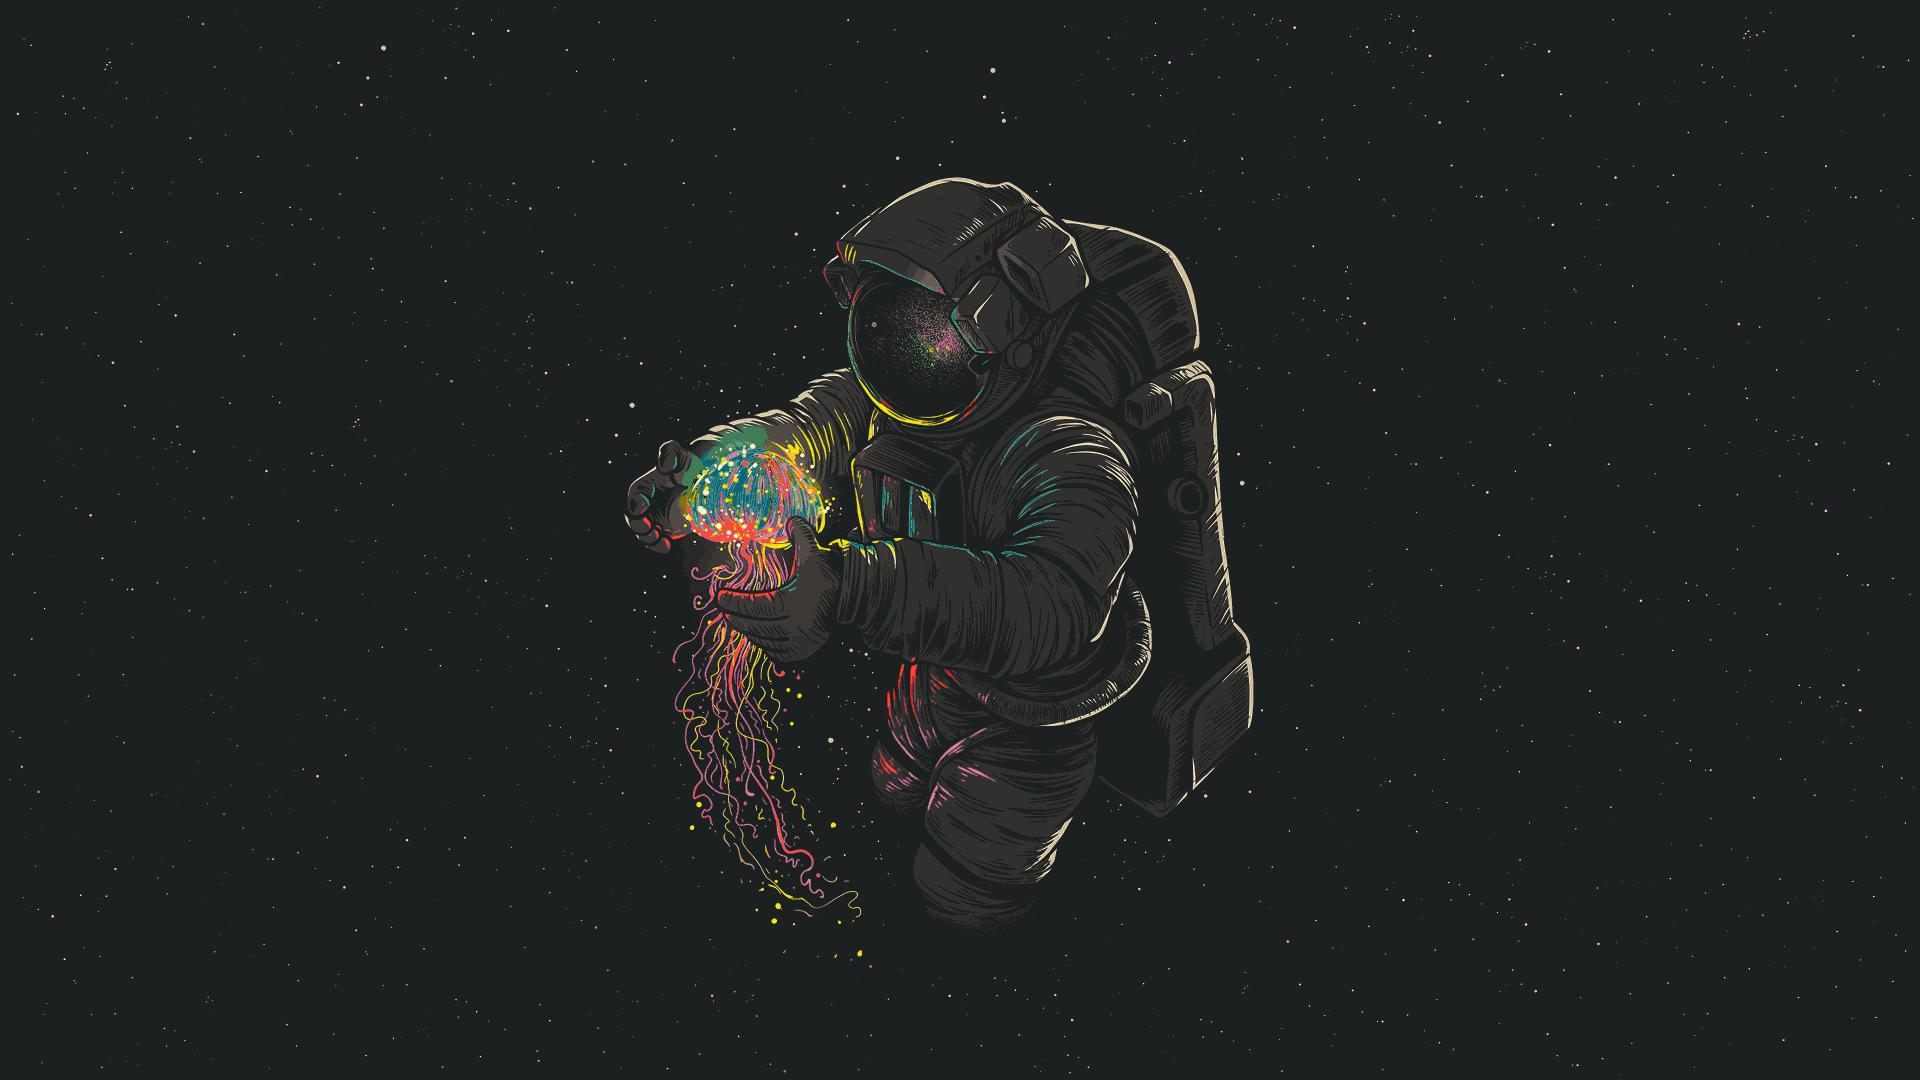
\includegraphics[width=10cm]{images/astronaut.png}
  \caption{\small{Um astronauta e uma água-viva}}
  \label{Astronauta}
\end{figure}

\newpage


\printbibliography % automatically generated

\section*{Referências}
\begin{itemize} % Itemize to create bullet list and enumerate order it
  \item Thomas Rintoul. Link here: <\url{https://youtu.be/nzXX2gc327M}>
  \item Jake B. Link here: <\url{https://youtu.be/lgiCpA4zzGU}>
  \item Detexify. Link here: <\url{https://detexify.kirelabs.org/classify.html}>
\end{itemize}

\end{document}
